\subsection{Kiến thức PCA (Principal Component Analysis) và (LDA) Linear Discriminant Analysis }

\subsubsection{PCA}
Giả sử ta có: $\langle x_1, x_2, \ldots, x_M \rangle_{N \times 1}$. Quá trình thực hiện giảm chiều tập dữ liệu trên bằng PCA được thực hiện qua các bước sau:
\begin{itemize}
	\item \textbf{Bước 1: }Tính các giá trị trung bình của các biến
	\begin{equation}
		\bar{x} = \frac{1}{M}\sum_{i=1}^{M}{x_i}
	\end{equation}
	\item \textbf{Bước 2: }Dời gốc tọa độ về điểm trung bình trong không gian dữ liệu.
	\begin{equation}
		\Phi_i = x_i - \bar{x}
	\end{equation}
	\item \textbf{Bước 3: }Tính ma trận hiệp phương sai:
	\begin{equation}
		C = \frac{1}{M}\sum_{m=1}^{M}{\Phi_m \Phi_m^T}
	\end{equation}
	\item \textbf{Bước 4: }Tính các trị riêng của C
	\begin{equation}
		\lambda_1 > \lambda_2 > \cdots > \lambda_N
	\end{equation}
	\item \textbf{Bước 5: }Tính các vector riêng tương ứng
	\begin{equation}
		u_1, u_2,\ldots,u_N
	\end{equation}
	\item \textbf{Bước 6: }Giữ lại K vector riêng có trị riêng tương ứng lớn nhất. Do ma trận hiệp phương sai đối xứng, nên các vector riêng đôi một song song nhau và tạo thành một hệ cơ sở. Ma trận chuyển không gian U được hình thành như sau:
	\begin{equation}
		U = \left[u_1, u_2, \ldots, u_K\right]
	\end{equation}
	\item \textbf{Bước 7: }Các điểm dữ liệu được chuyển qua không gian mới (có số chiều K << N) theo công thức:
	\begin{equation}
		b = U^T\left(x - \bar{x}\right)
	\end{equation}
\end{itemize}
\pagebreak

\textit{Ví dụ minh họa:}
Có các điểm sau (2.5, 2.4), (0.5, 0.7), (2.2, 2.9), (1.9, 2.2), (3.1,3.0), (2.3, 2.7), (2, 1.6), (1, 1.1), (1.5, 1.6), (1.1, 0.9). Sử dụng PCA để giảm chúng về 1 chiều.
\begin{itemize}
    \item \textbf{Bước 1:} Tính trung bình, chuẩn hóa.
    \begin{figure}[H]
        \begin{center}
            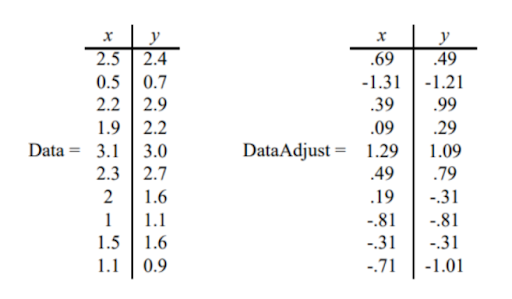
\includegraphics[scale=0.7]{images/theo2/PCA-cal-1}
            \caption{Tính trung bình, chuẩn hóa}
        \end{center}
    \end{figure}

    \item \textbf{Bước 2:} Ma trận hiệp phương sai.
    \begin{figure}[H]
        \begin{center}
            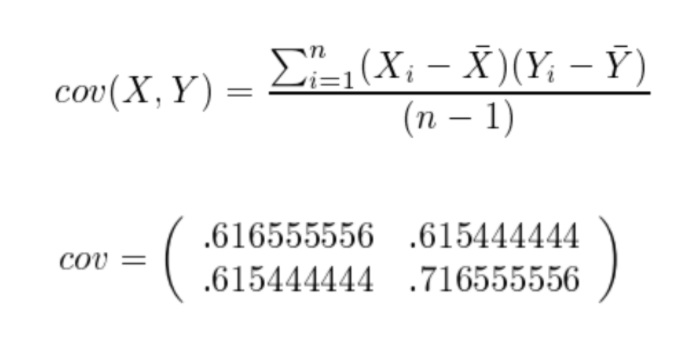
\includegraphics[scale=0.4]{images/theo2/PCA-cal-2}
            \caption{Ma trận hiệp phương sai}
        \end{center}
    \end{figure}

    \item \textbf{Bước 3:} Tính vector riêng và giá trị riêng cho ma trận hiệp phương sai.
    \begin{figure}[H]
        \begin{center}
            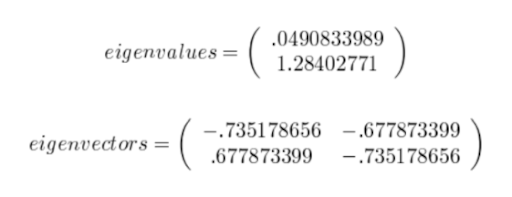
\includegraphics[scale=0.5]{images/theo2/PCA-cal-3}
            \caption{Ma trận hiệp phương sai}
        \end{center}
    \end{figure}
    
    \item \textbf{Bước 4:} Biến đổi dữ liệu:
    \begin{figure}[H]
        \begin{center}
            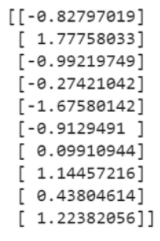
\includegraphics[scale=0.5]{images/theo2/PCA-cal-4}
            \caption{Dữ liệu sao khi biến đổi}
        \end{center}
    \end{figure}
\end{itemize}

\subsubsection{LDA}

\begin{itemize}
    \item \textbf{Bước 1:} Tính ma trận phân tán giữa các nhóm.
    \begin{equation}
        S_B=\sum_{i=1}^{C}{c_i(\mu_i - \mu)(\mu_i-\mu)^T}
    \end{equation}
    \subitem $\mu_i$ là giá trị trung bình của từng lớp. 
    \subitem $\mu$ là giá trị trung bình của tất cả dữ liệu. 

    \item \textbf{Bước 2:} Tính ma trận phân tán tích lũy ứng với từng nhóm.
    \begin{equation}
        S_W=\sum_{j=1}^{C}{\sum_{i=1}^{n_j}{(x_{ij}-\mu_j)(x_{ij}-\mu_j)^T}}
    \end{equation}

    \item \textbf{Bước 3:} Xây dựng hàm tiêu chí tách lớp.
    \begin{equation}
        W = S_W^{-1}S_B
    \end{equation}

	\item \textbf{Bước 4:} Tính các vector riêng (chọn ra tối đa C - 1 vector riêng có giá trị riêng tương ứng lớn nhất) của W. Từ đó hình thành ma trận đổi cơ sở:
	\begin{equation}
		U = \left[w_1, w_2, \ldots, w_{C-1}\right]
	\end{equation}

	\item \textbf{Bước 5:} Chuyển các điểm dữ liệu sang không gian mới
	\begin{equation}
		y = U^T(x - \mu)
	\end{equation}
\end{itemize}
\pagebreak

\textit{Ví dụ:} Cho tập dữ liệu:
$$
X = \left( \begin{array}{cc}
	4 & 1 \\
	2 & 4 \\
	2 & 3 \\
	3 & 6 \\
	4 & 4 \\
	9 & 10 \\
	6 & 8 \\
	9 & 5 \\
	8 & 7 \\
	10 & 8 \\

\end{array} \right)
%
y = \left( \begin{array}{c}
	1 \\
	1 \\
	1 \\
	1 \\
	1 \\
	2 \\
	2 \\
	2 \\
	2 \\
	2 \\
\end{array} \right)
$$

\textit{Ta có:} 
$$
\mu_1 = \left( \begin{array}{c}
	3.0 \\
	3.6
\end{array} \right)
%
\mu_2 = \left( \begin{array}{c}
	8.4 \\
	7.6	
\end{array} \right)
\mu = \left( \begin{array}{c}
	5.7 \\
	5.6	
\end{array} \right)
$$

\begin{itemize}
	\item \textbf{Bước 1:} Tính $S_B$
	$$
		S_B = \left( \begin{array}{cc}
			29.16 & 21.6\\
			21.6 & 16.0
		\end{array}\right)
	$$
	\item \textbf{Bước 2:} Tính $S_W$
	$$
		S_W = \left( \begin{array}{cc}
			2.64 & -0.44\\
			-0.44 & 5.28
		\end{array}\right)
	$$
	\item \textbf{Bước 3:} Tìm ma trận chuyển không gian, bước này tượng tự với các bước từ bước 3 trở về sau của PCA nhưng thay ma trận C bằng ma trận $W = S_W^{-1}S_B$
	$$
		\lambda = 15.65 
		\Longrightarrow w = \left( \begin{array}{c}
			0.91\\
			0.39
		\end{array}\right)
	$$
	\item \textbf{Bước 4:} Chuyển các điểm dữ liệu về không gian mới ($b = w^Tx$)
	$$
		\left( \begin{array}{c}
			4.03 \\
			3.38 \\
			2.99 \\
			5.07 \\
			5.2 \\
			12.09 \\
			8.58 \\
			10.14 \\
			10.01 \\
			12.22 \\
		\end{array} \right)
	$$
\end{itemize}
\pagebreak

\subsubsection{Sự khác biệt giữa PCA và LDA}
\begin{itemize}
	\item PCA giảm chiều dữ liệu không quan tâm đến lớp của dữ liệu đó (Unsupervised Learning). Trong khi LDA lại quanh tâm đến lớp của các điểm dữ liệu (Supervised Learning).
	\item PCA giảm chiều xuống một giá trị K nhỏ hơn số thuộc tính của dữ liệu. Trong khi LDA chỉ có thể  giảm số chiều sao cho số chiều giảm xuống phải nhỏ hơn số lớp trong tập dữ liệu.
	\item LDA sẽ cho kết quả tốt hơn trên tập huấn luyện vì có quan tâm đến nhãn.
	\item LDA dễ gặp các trường hợp suy biến khi chiều ban đầu của dữ liệu rất lớn như số lượng điểm dữ liệu trong tập lại quá nhỏ. Ví như các dữ liệu ảnh.
\end{itemize}
\begin{figure}[H]
	\begin{center}
		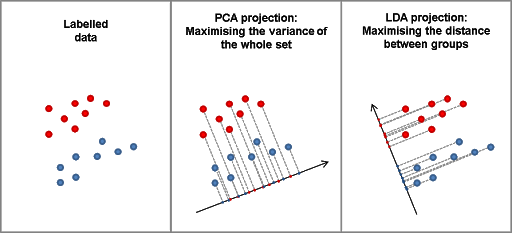
\includegraphics[scale = 0.5]{images/theo2/LDA-PCA-cmp}
		\caption{So sánh LDA và PCA}
	\end{center}
\end{figure}